\documentclass{article}
\usepackage{style-notes}

\newcounter{lecnum} 	% define counter for lecture number
\renewcommand{\thepage}{\thelecnum-\arabic{page}}	% define how page number is displayed (< lecture number > - < page number >)

% define lecture header and page numbers
% NOTE: to call use \lecture{< Lecture # >, < Lecture name >, < Chapter # >, < Chapter name >, < Section #s >}
\newcommand{\lecture}[5]{

    % define headers for first page
    \thispagestyle{empty} % removes page number from page where call is made

    \setcounter{lecnum}{#1}		% set lecture counter to argument specified

    % define header box
    \begin{center}
    \framebox{
      \vbox{\vspace{2mm}
    \hbox to 6.28in {\textbf{MATH 320: Probability} \hfill}
       \vspace{4mm}
       \hbox to 6.28in {{\hfill \Large{Lecture #1: #2} \hfill}}
       \vspace{2mm}
       \hbox to 6.28in {\hfill Chapter #3: #4 \small{(#5)}}
      \vspace{2mm}}
    }
    \end{center}
    \vspace{4mm}
    
    % define headers for subsequent pages
    \fancyhead[LE]{\textit{#2} \hfill \thepage} 		% set left header for even pages
    \fancyhead[RO]{\hfill \thepage}		% set right header for odd pages

}

% define macros (/shortcuts)
\newcommand{\bu}[1]{\textbf{\ul{#1}}}				% shortcut bold and underline text in one command
\newcommand{\blankul}[1]{\rule[-1.5mm]{#1}{0.15mm}}	% shortcut for blank underline, where the only option needed to specify is length (# and units (cm or mm, etc.)))
\newcommand{\comp}{{\sim}}		% shortcut for tilde without extra space, using for complement
\newcommand{\vectwo}[2]{#1_1, \ldots, #1_{#2}}	% define vector (without parentheses, so when writing out in like a definition) of the form X_1, ..., X_k, where X and k are variable. NOTE: to call use $\vectwo{X}{k}$
\newcommand{\follow}[1]{\sim \text{#1}\,}		% shortcut for ~ 'Named dist ' in normal font with space before parameters would go
\newcommand{\followsp}[2]{\overset{#1}\sim \text{#2}\,}		% (followsp is short for 'follow special') shortcut that can be used for iid or ind ~ 'Named dist ' in normal font with space before parameters would go
\newcommand{\ind}{\perp \!\!\! \perp}		% define independence symbol (it basically makes two orthogonal symbols very close to each other; the number of \! controls the space between each of the orthogonal symbols)
\newcommand{\e}{\mathrm{e}}		% shortcut for non-italic e in math mode



% NOTES on what didn't cover
% random sample of bernoulli to get binomial (textbook 2.4 and lazar)
% algebraic derivation of binomial E(X) (Theory lecture 8)
% derivation of geometric mean (Lazar notes, 2.2), actex 5.4.2 has a much easier geometric mean derivation (but it's with the other way to write geometric dist, so would have to rework)
% in textbook (section 2.5, neg binom), they derive geometric probabilities a different way than in theory (lazar has this derivation written out better). They derived P(X > x) using geometric sums, then did F(X) = 1 - P(X > x). Should understand that for my own notes

% Fancy reason why negative binomial is called negative binomial (explanation in 2.6 (10th edition) of the text)

% Informal derivation of poisson pmf (FA 22 notes common used discrete part 3 and theory lecture 10-4)
% -> written explanation of the relationship between poisson and binomial
% -> poisson approximation to the binomial
% -> don't think all above is super relevant for exam P or baby theory, leave for grad school
% Formal derivation of poisson pmf from binomial (theory lecture 10-4)

\begin{document}

\lecture{10}{Discrete Distributions}{2}{Distributions}{2.1, 2.3, 2.4, 2.5, 2.6, 2.7}


\bu{Introduction}\bigskip

\begin{itemize}
    \item Statistical distributions are used to model \blankul{3cm}.
    \item[] We usually deal with a \textbf{family} of distributions rather than a single distribution (family = type of distribution).
    \item This family is indexed by one or more \blankul{3cm}, which allows us to vary certain characteristics of the distribution while staying with one functional form.
    \item[] The functional form determines the unique features of the distribution.
    \item For example, if the distribution of a population of symmetric and bell-shaped, then a \blankul{2cm} distribution is a reasonable choice. Then we will specify the parameters \blankul{2cm}.\bigskip
    \item In the previous sections, we saw a number of examples of discrete probability distributions.
    \item[] Recall a random variable $X$ is said to have a discrete distribution if \blankul{3cm} is countable.
    \item In the next sections we will study some special distributions that are extremely useful and widely applied, some of which we have already seen before.
\end{itemize}\bigskip

\bu{Discrete uniform distribution}\bigskip

Definition\bigskip
\begin{itemize}
    \item Scenario: If a finite number of values are equally likely to be observed, then a discrete uniform distribution is used to model.\bigskip
    \item Definition: A random variable $X$ has a \textbf{discrete uniform} ($N_0, N_1$) distribution if
    \[P(X = x \mid N_0, N_1) = \frac{1}{N_1 - N_0 + 1}, \quad\quad\quad x = N_0, \ldots, N_1,\]
    \item[] where $N_0$ and $N_1$ are specified integers ($N_0 \le N_1$).
    \item If $X$ follows a discrete uniform (DU) distribution with parameters $N_0$ and $N_1$, we can summarize this using the following notation:
    \[\text{RV}\follow{Distribution}(\text{parameters}) \hspace{20pt} X \follow{Discrete uniform}(N_0, N_1)\]
    \item[] ``The random variable $X$ \textbf{follows} (is distributed as / assumed to have) a discrete uniform distribution with parameters $N_0$ and $N_1$''.
    \item[] Can also use this more generally with $X \follow{$F_X(x)$}$ or $X \follow{$f_X(x)$}$.
    \item Example: Rolling a fair 6-sided die.\bigskip
    \item[] $P(X = x \mid N_0, N_1) = $\bigskip
    \item A note on notation: When we are dealing with parametric distributions, the distribution is dependent on the values of the parameters. In order to emphasize this fact and keep track of the parameters, write them in the pmf preceded by: $\mid$ (given).
    \item[] In general, we have $P(X = x \mid \theta)$, where $\theta$ could be a vector of parameters.
\end{itemize}\bigskip

Mean and variance\bigskip
\begin{itemize}
    \item One of the advantages of having families of distributions is that the pmfs have the same functional form (i.e. follow a certain pattern). This is also true for their expected value and variances.
    \item If a random variable $X$ has a discrete uniform distribution $(N_0, N_1)$,\smallskip
    \[E(X) = \frac{N_0 + N_1}{2} \hspace{80pt} V(X) = \frac{(N_1 - N_0 +1)^2 -1}{12}\]
    \item The mean and variance are functions of the parameters.
    \item Continuing example: Find the mean and variance of rolling a fair 6-sided die.
    \item[] Use formulas: \hspace{150pt} Confirm with definition:\vspace{60pt}
\end{itemize}\bigskip

Summary\bigskip
\begin{itemize}
    \item If we know (or assume) the family of a distribution and the values of the parameters
    \item[] $\Longleftrightarrow$ know \blankul{2cm} $\Longleftrightarrow$ \blankul{2cm}
    \item[] We also know the expected value and variance as well.
    \item This statement works backwards too.
    \item \textit{IMPORTANT STRATEGY} when solving problems:
    \item[] If we recognize that we have a pmf where the the range of the random variable and the probabilities match the scenario of a specific distribution, then that random variable must follow that specific distribution.\bigskip
    \item Examples: How can we model the following populations?
    \begin{enumerate}
        \item Suppose $f_X(x) = \frac{1}{4}, \quad x = 7, 8, 9, 10$\vspace{60pt}
        \item[] Find $E(X^2)$.\vspace{60pt}
        \item Suppose the values 3, 6, 9, 12, 15 are equally likely.\vspace{30pt}
        \item Suppose the values 5, 9, 13, 17 are equally likely.\vspace{30pt} 
    \end{enumerate}
\end{itemize}\bigskip

\bu{Bernoulli distribution}\bigskip

Motivation\bigskip
\begin{itemize}
    \item The following four distributions are constructed based on Bernoulli experiments: \\Binomial, Geometric, Hypergeometric, Negative Binomial.
    \item Example experiments:
    \begin{enumerate}
        \item Produce a product and see if the product is defective.
        \item Roll a die and see if a number greater than 4 appears.
        \item Choose a student in this class at random and see if a female student is chosen.
    \end{enumerate}
    \item What is the common characteristic of these experiments?\bigskip
    \item The main event of interest is labeled \blankul{2.5cm} and the other is labeled \blankul{2.5cm}.
\end{itemize}\bigskip

Definition\bigskip
\begin{itemize}
    \item Scenario: The random variable for which 0 and 1 are chosen to describe the two possible values is called a \textbf{Bernoulli random variable}.
    \item The outcomes in Success and Failure are assigned \blankul{1cm} and \blankul{1cm} by the Bernoulli random variable, respectively.\vspace{80pt}
    \item Definition: A random variable $X$ has a \textbf{Bernoulli} $(p)$ distribution if
    \[
    P(X = x \mid p) =
        \left\{
        \begin{array}{ll}
            1 - p \hspace{15pt} & \quad x = 0\\
            p & \quad x = 1\\
            0 & \quad \text{otherwise}\\
        \end{array}
        \right.
    \]
    \item[] where the parameter $p$ represents the probability of success and $0 < p < 1$.
    \item[] Equivalently, $f(x \mid p) = p^x (1 - p)^{1 - x}, \quad x = 0,1$.\bigskip
    \item Notation: $X \follow{Bernoulli}(p)\bigskip$
    \item Example: A basketball player shoots a free throw with a 75\% probability of success. Let $X$ denote the number of points scored.
    \begin{enumerate}[(a)]
        \item What is the distribution of $X$?\vspace{30pt}
        \item Find the pmf of $X$.\vspace{35pt}
        \item Find the expected value of $X$ (by hand using the definition).\vspace{80pt}
        \item Find the variance of $X$ (by hand using the definition).\vspace{80pt}
    \end{enumerate}
\end{itemize}\bigskip

Mean and variance\bigskip
\begin{itemize}
    \item If $X \follow{Bernoulli}(p)$\smallskip
    \[E(X) = p \hspace{80pt} V(X) = p(1 - p) = pq\]
    \item Derive $E(X)$. \textit{HINT}: Generalize the calculations from the previous examples.\vspace{80pt}
    \item Derive $V(X)$.\vspace{170pt}
    \item[] ** We can always try to derive the mean and variance of distributions by going back to the definitions.
\end{itemize}\bigskip

\bu{Binomial distribution}\bigskip

Motivation\bigskip
\begin{itemize}
    \item Example experiments:
    \begin{enumerate}
        \item A basketball player gets 10 3-point shots and has a probability of success (making a basket) of 1/5. Let $X$ be the number of makes out of the 10 attempts.
        \item A factory produces 100 products with the probability of defect 2/100. Let $Y$ be the number of defective products out of 100 products.
        \item Roll a fair die 3 times. Let $Z$ be the number of 6s out of the 3 rolls.
    \end{enumerate}
    \item What is the common characteristic of these experiments?
\end{itemize}\bigskip

Binomial experiments and binomial random variables\bigskip
\begin{itemize}
    \item Definition: An experiment is called a \textbf{binomial experiment} if all of the following hold:\bigskip
    \item[] These are the conditions needed in order to have a binomial experiment.
    \begin{enumerate}
        \item The experiment consists of a fixed number, $n$, of identical trials.
        \item[] (Note that \textbf{identical} = from the same family with the same parameter values.)
        \item Each trial results in one of two events: success or failure.
        \item There is a constant probability of success, $p$, for each trial.
        \item The trials are independent.
        \item The outcome is a sequence of successes and failures.
    \end{enumerate}\bigskip
    \item[] Said another way, a binomial experiment is a sequence of \blankul{5cm}.
    \item Definition: If $X$ is the number of successes in a binomial experiment, $X$ is called a \textbf{binomial random variable}.\bigskip
    \item Examples:
    \begin{enumerate}[(a)]
        \item Check the conditions to determine if example experiment 1 is indeed a binomial experiment.\vspace{200pt}
        \item Are the conditions met for experiments 2 and 3? If so, identify $n$ and $p$.\vspace{50pt}
    \end{enumerate}
\end{itemize}\bigskip

Binomial probabilities\bigskip
\begin{itemize}
    \item Probabilities for binomial distribution are just an application of the multiplication rule for independent event.
    \item Example: Lets say our basketball player has only 3 shot attempts now. Lets visualize the tree diagram illustrating the different outcomes of this binomial experiment\\ ($M = $ make, $\comp{M} = $ miss).
    \begin{figure}[H]
        \center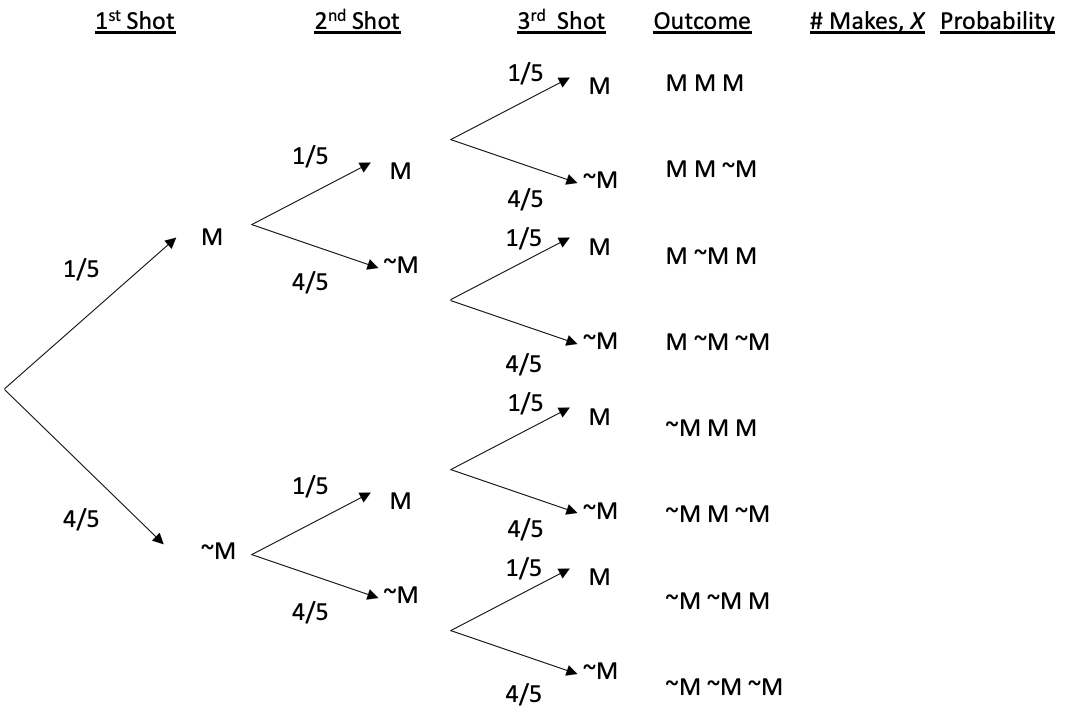
\includegraphics[scale=0.75]{test-3/binomial-tree-diagram}
    \end{figure}
    \begin{enumerate}[(a)]
        \item Find $P(X = 3)$.\vspace{50pt}
        \item Find $P(X = 2)$.\vspace{50pt}
        \item[] Another way to think about the number of branches:
        \item[] \blankul{3cm} that include exactly 2 makes.
        \item[] This could also be found using \blankul{4cm}.
        \item Now suppose $n = 8$. Find $P(X = 4)$.
        \item[] \hspace{10pt} = \hspace{10pt} sequences = \hspace{10pt} ways to choose 4 success out of the $n = 8$ trials.
        \item[] Now just need the probability of 4 success and 4 failures:\vspace{30pt}
    \end{enumerate}
    \item We can use these patterns to obtain a general formula for the $P(X = x)$ for a binomial random variable with $(n, p)$.
\end{itemize}\bigskip

Definition\bigskip
\begin{itemize}
    \item Definition: A random variable $X$ has a \textbf{binomial} distribution based on $n$ trials with success probability $p$ if the pmf of $X$ has the form
    \[P(X = x \mid n, p) = {n \choose x}\, p^x\, (1 - p)^{n - x}, \quad\quad\quad x = 0, 1, \ldots, n\]\vspace{20pt}
    \item[] where $0 < p < 1$ and $n$ is an integer such that $n \ge 1$.\smallskip
    \item Notation: $X \follow{Binomial}(n, p)$\bigskip
    \item Example: Suppose a student is taking a multiple choice exam with 15 questions (4 choices each). They will be randomly guessing on each question. Let $X$ be the number of questions out of 15 for which the student guesses correctly.
    \begin{enumerate}[a)]
        \item What is the distribution of $X$?\vspace{40pt}
        \item Find the pmf of $X$.\vspace{50pt}
        \item Find $P(X = 7)$.\vspace{50pt}
        \item Find the probability of at least one correct.\vspace{50pt}
        \item Find $P(X < 6)$.\vspace{50pt}
        \item Find $P(X \ge 6)$.\vspace{50pt}
    \end{enumerate}
    \item Binomial cdf:\bigskip
    \item[] Right sided probability:
\end{itemize}\bigskip

Mean and variance\bigskip
\begin{itemize}
    \item If $X \follow{Binomial}(n, p)$\smallskip
    \[E(X) = np \hspace{80pt} V(X) = np(1 - p) = npq\]
    \item Continuing example:
    \begin{enumerate}[(a)]\setcounter{enumi}{5}
        \item Find the expected value and variance of the number of questions guessed correctly.\vspace{60pt}
        \item Suppose each question is worth 4 points. Find the expected value and variance of the number of points missed on the exam if it is worth a total of 60 points.
        \begin{itemize}
            \item[*] $X = $ number of question correct:
            \item[*] $Y = $ number of points earned:
            \item[*] $Z = $ number of points missed:
        \end{itemize}\vspace{40pt}
    \end{enumerate}
\end{itemize}

\newpage

More examples\bigskip
\begin{enumerate}
    \item A coin is weighted so that the probability of flipping heads is 0.65. The coin is flipped 10 times and each flip is independent of every other flip. Let $X$ be the the number of heads in the 10 flips.
    \begin{enumerate}
        \item Give the pmf of $X$, $\mu_X$ and $\sigma_x^2$.\vspace{30pt}
        \item Find: $P(X = 3)$ \hfill $P(X < 3)$ \hfill $P(X \ge 3)$.\vspace{80pt}
        \item If $Y = 10 - X$ give the distribution of $Y$. Find $P(Y \le 1)$.\vspace{70pt}
    \end{enumerate}
    \item A hospital obtains 40\% of its flu vaccine shipments from Company A, 50\% from Company B, and 10\% from Company C.
    \item[] From manufacturing specifications, it is known that 3\% of the vials from A are ineffective, 2\% from B are ineffective, and 5\% from C are ineffective.
    \item[] The hospital tests five vials from each large shipment from a company. If at least one of the five is ineffective, find the conditional probability of that shipment having come from C.\vspace{200pt}
\end{enumerate}

Relationship between Bernoulli and binomial\bigskip
\begin{itemize}
    \item We can think of the result of a binomial experiment as a sequence of 0s and 1s with length $n$, where each individual number is the result of a Bernoulli experiment.
    \item $X$ is the number of successes. Take $n = 5$ for example. We could have:
    \item[] $(0,0,1,0,0)$
    \item[] $(1,0,1,1,0)$
    \item[] $(1,1,1,1,1)$\bigskip
    \item Suppose that $X \follow{Bin}(n, p)$ and $\vectwo{Y}{n} \followsp{\ind}{Ber}(p)$ $\Longleftrightarrow$ $Y_i \followsp{iid}{Ber}(p)$ where \\$iid = $ independent and identically distributed.
    \[X = \]
    \item[] Bernoulli distribution is a special case of Binomial when 
    \item[] This is intuitively obvious and can be verified in the distribution formula as well.
    \item Compare the expected values and variances.
    \item[] Note that the expected value of a sum is the \blankul{6cm}.\vspace{60pt}
\end{itemize}\bigskip

Visualizing binomial distributions\bigskip

\begin{figure}[H]
    \center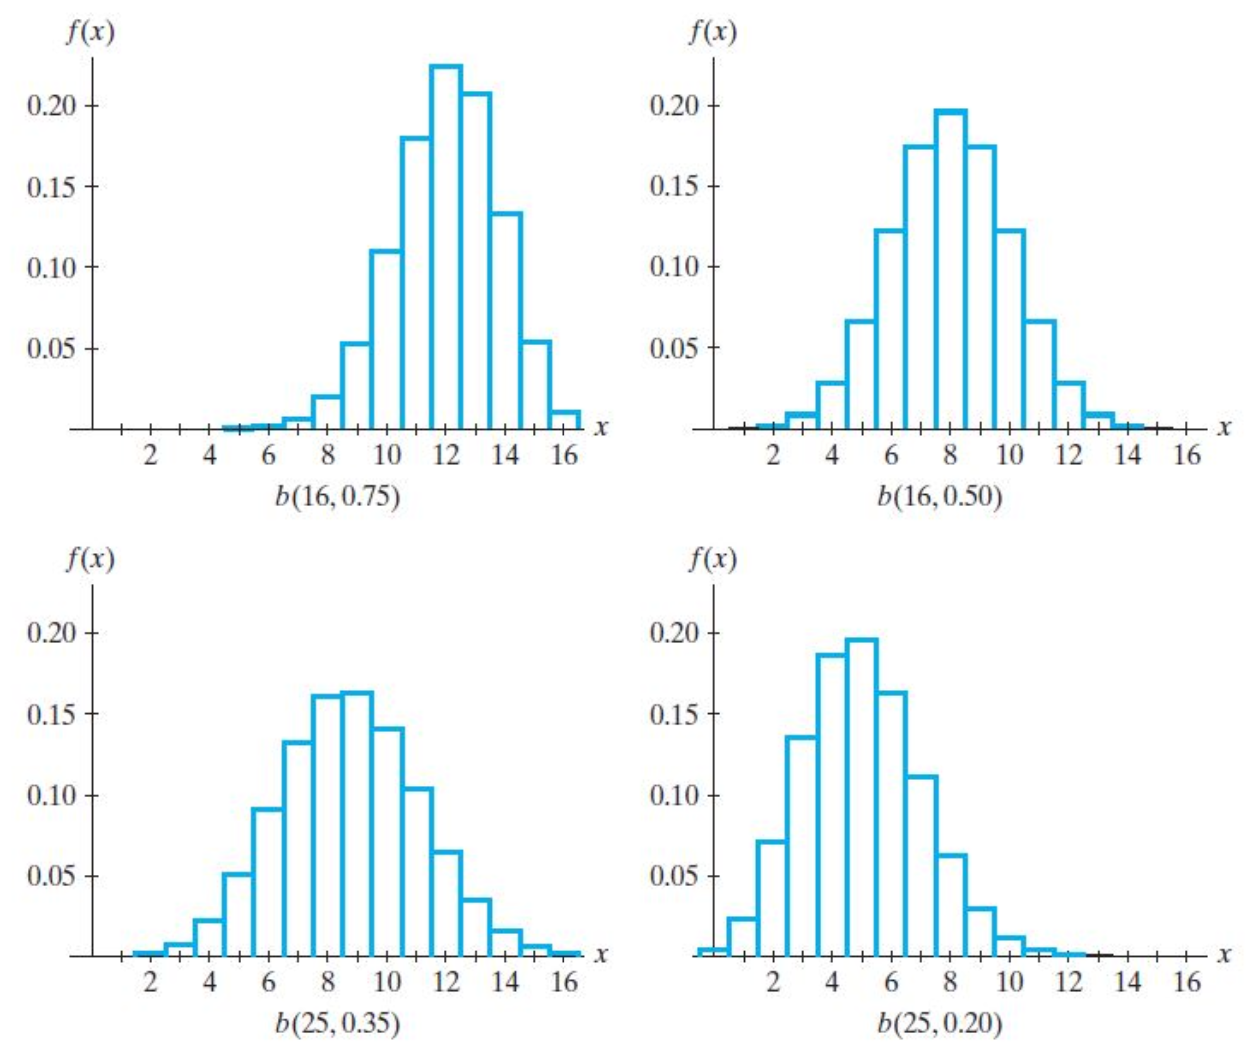
\includegraphics[scale=0.4]{test-3/binomial-pmfs}
\end{figure}

\bu{Geometric distribution}\bigskip

Motivation\bigskip
\begin{itemize}
    \item Example experiments:
    \begin{enumerate}
        \item A basketball player shoots three pointers (with success probability of 1/5) until they make the first one. Let $X$ be the number of shots it took to make the first one.
        \item An oil prospector will drill a succession of holes in a given area to find a productive well. He stops when he finds a productive well. Let $Y$ be the number wells drilled before the first productive well.
        \item Roll a fair die until the number 6 appears. Let $Z$ be the number of rolls to get the first 6.
    \end{enumerate}
    \item What is the common characteristic of these experiments?
\end{itemize}\bigskip

Geometric experiments and geometric random variables\bigskip
\begin{itemize}
    \item The general setting for a geometric distribution problem has many features in common with a binomial distribution problem.
    \item Characteristics of a \textbf{geometric experiment}.\smallskip
    \begin{enumerate}
        \item Each trial is a Bernoulli experiment.
        \item The trials are identical and independent.
        \item The sample space is: $S = $
    \end{enumerate}\smallskip
    \item Geometric is a waiting time random variable, with the number of successes fixed at 1.
    \item There are TWO forms of a \textbf{geometric RV}. \ul{We will be using the FIRST}.\smallskip
    \begin{itemize}
        \item These are just two different ways to interpret outcomes in the sample space (i.e. define the range of the random variable).
    \end{itemize}
    \begin{enumerate}
        \item The random variable of interest $X$ is the number of trials.\bigskip
        \item The random variable of interest $Y$ is the number of failures before the first success.
    \end{enumerate}\bigskip
    \item Relationship between the two formulations.
    \begin{itemize}
        \item The first way $X$ includes the trial on which the success occurs, whereas the second way $Y$ does not.\bigskip
        \item This obviously will result in the pmf, expected value, etc. being different between $X$ and $Y$.
    \end{itemize}
    \item Example: Check the conditions to determine if example experiment 1 is indeed a geometric experiment.\vspace{30pt}
\end{itemize}\bigskip

Definition\bigskip
\begin{itemize}
    \item Informal derivation of the pmf: We can use the multiplication rule of independent events to find the probability of $x$ trials to get the first success.\bigskip
    \begin{enumerate}
        \item Success on first trial:\bigskip
        \item Success on second trial:\bigskip
        \item Success on third trial:\bigskip
    \end{enumerate}\vspace{40pt}
    \item If $X \follow{Geometric}(p)$,
    \[P(X = x \mid p) =  \]\bigskip
    \item[] Alternate form: $Y = $\bigskip
\end{itemize}\bigskip

Mean and variance\bigskip
\begin{itemize}
    \item If $X \follow{Geometric}(p)$,
    \[E(X) = \frac{1}{p}, \hspace{80pt} V(X) = \frac{1 - p}{p^2} = \frac{q}{p^2}\]\bigskip
    \item[] Alternate form:\bigskip
    \item Continuing example: Let $X \sim \text{Geometric}(p = 1/5)$. How many trials do you expect to see the first success (make)?
\end{itemize}

\newpage

Geometric probabilities\bigskip
\begin{itemize}
    \item A geometric random variable is a geometric series:\vspace{30pt}
    \item \textbf{Sums of geometric series}: We will use these properties to derive formulas for geometric probabilities.
    \item[] Let $q$ be a real number such that $\lvert q \rvert < 1$, and let $m$ be any positive integer $m \ge 1$. 
    \begin{itemize}
        \item Infinite geometric series:
        \item[] $\displaystyle\text{(a)}\quad \sum_{i = 0}^{\infty} q^i= q^0 + q^1 + q^2 + \dots = \frac{1}{1 - q} \hspace{20pt} \text{(b)}\quad \sum_{i = 1}^{\infty} q^i = \frac{q}{1 - q}$\bigskip        \item[] \textit{PATTERN}: Numerator = \blankul{4cm} and denominator = \blankul{4cm}.\bigskip
        \item Another sum:
        \item[]$\displaystyle \text{(c)} \quad \sum_{i = 0}^{m} q^i = $\vspace{50pt}
    \end{itemize}
    \item By these sums of a geometric series, we can compute the following probabilities. For positive integers $x$, $a$, and $b$ such that $a < b$.
    \begin{itemize}
        \item Total probability: $P(X < \infty) = \hspace{10pt}$.
        \item[] Derive this:\vspace{150pt}
        \item Cdf: $P(X \le x) = $\vspace{150pt}
        \item[] Intuitive derivation of cdf:\vspace{100pt}
        \item Right probability (exclusive): $P(X > x) = $\vspace{70pt}
        \item Right probability (inclusive): $P(X \ge x) = $\vspace{70pt}
        \item Interval probability: $P(a < X \le b) = $\vspace{70pt}
        \item Interval probability (both inclusive): $P(a \le X \le b) = $\vspace{40pt}
    \end{itemize}
   
    \item Example: Suppose that the probability of engine malfunction during any one-hour period is $p = 0.02$. Let $X$ be the number of one-hour intervals until the first malfunction.
    \begin{enumerate}[a)]
        \item What is the distribution of $X$?\vspace{40pt}
        \item Find the pmf of $X$.\vspace{40pt}
        \item Find the probability that an engine will survive 3 hours.\vspace{40pt}
        \item Find the probability that an engine will survive 3 hours, but die before or during the 6\textsuperscript{th} hour.\vspace{50pt}
        \item Suppose that an engine survives 3 hours. Find the probability that the engine will survive 6 hours.\vspace{40pt}
    \end{enumerate}
\end{itemize}\bigskip

Memoryless property\bigskip
\begin{itemize}
    \item The geometric distribution has an interesting property, known as the ``memoryless'' property. For integers $s > t$, it is the case that
    \[P(X > s \mid X > t) = P(X > s - t)\]
    \item To help us understand what this means, let's interpret some events for $s > t$.
    \begin{itemize}
        \item $\{X > s\}$\smallskip
        \item $\{X > t\}$\smallskip
        \item $\{X > s\} \mid \{X > t\}$\bigskip
    \end{itemize}
    \item For example, lets say I flip a coin three times and don't get a tails. Do these past failures help to increase the probability of getting a tails next?\vspace{30pt}
    \item We want to know how (if it all) this past information influences the future event. Recall $P(X > a) = q^a$.
    \item[] $P(X > s \mid X > t) = $\vspace{120pt}
    \item The probability of getting an additional failures $s - t$, having already observed $t$ failures is the same probability of observing $s - t$ failures at the start of the sequence.\vspace{140pt}
    \item That's why this property is called the memoryless property. Even though we have some failures before, a geometric experiment is sort of restarting again. Thus, the geometric distribution ``forgets'' what has occurred.
\end{itemize}\bigskip

Visualizing geometric distributions\bigskip

\begin{figure}[H]
    \center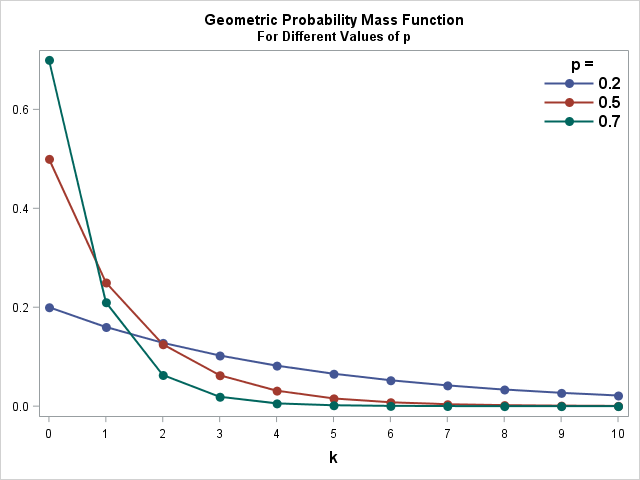
\includegraphics[scale=0.4]{test-3/geometric-pmfs}
\end{figure}

\newpage

\bu{Negative binomial distribution}\bigskip

Motivation\bigskip
\begin{itemize}
    \item Example experiments:
    \begin{enumerate}
        \item A basketball player shoots three pointers (with success probability of 1/5) until they make the 4 shots. Let $X$ be the number of shots it took to make the 4\textsuperscript{th} one.
        \item An oil prospector will drill a succession of holes in a given area to find a productive well. He stops when he finds three productive wells. Let $Y$ be the number wells drilled before the 3\textsuperscript{rd} productive well.
    \end{enumerate}
    \item What is the common characteristic of these experiments?\bigskip
\end{itemize}\bigskip

Negative binomial experiments and negative binomial random variables\bigskip
\begin{itemize}
    \item The negative binomial experiment is a generalized version of the geometric experiment.
    \item Characteristics of a \textbf{negative binomial experiment}.\smallskip
    \begin{enumerate}
        \item Each trial is a Bernoulli experiment.
        \item The trials are identical and independent.
        \item The number of successes to stop a negative binomial experiment is denoted by $r$.
        \begin{itemize}
            \item This is a parameter of the distribution.
        \end{itemize}
    \end{enumerate}\smallskip
    \item \textbf{Negative binomial random variable}.
    \begin{itemize}
        \item[] (Following the logic from the geometric distribution, there is also two ways to define a negative binomial random variable. We will only discuss the one corresponding to the version of the geometric we are using.)\smallskip
        \item The random variable of interest $X$ is the number of trials until $r$ successes.
        \item Simple demonstration of the random variable mapping: When $r = 3$, the sample space and range are:\vspace{50pt}
        \item In general, the range of $X$ is\vspace{15pt}
    \end{itemize}
    \item Example: Check the conditions to determine if example experiment 1 is indeed a negative binomial experiment.\vspace{30pt}
\end{itemize}\bigskip

Definition\bigskip
\begin{itemize}
    \item Informal derivation of the pmf: We can again use the multiplication rule of independent events to find the probability of $x$ trials to get $r$ successes.\bigskip
    \begin{enumerate}
        \item The outcomes in the event $\{X = x\}$ must follow these two rules:
        \begin{enumerate}[A)]
            \item The first $x - 1$ trials result in $r - 1$ successes and $x - r$ failures.
            \item The last $x$\textsuperscript{th} trial has to result in success.
        \end{enumerate}\bigskip
        \item Lets visualize these rules (and think of them as events) to get some probabilities.
        \begin{itemize}
            \item Consider a sequence of Bernoulli trials with probability of success $p$,\\ $0 < p < 1$. Let $x = r, r + 1, \ldots$.\vspace{90pt}
        \end{itemize}
        \begin{enumerate}[A)]
            \item $A \sim$
            \item[] $P(A) = $\bigskip
            \item $B \sim$
            \item[] $P(B) = $\bigskip
        \end{enumerate}
        \item Putting these together:\bigskip
        \item[] $f_X(x \mid r, p) = P(A \cap B) = $\vspace{40pt}
    \end{enumerate}
    \item If $X \follow{Negative binomial}(r, p)$,
    \[P(X = x \mid r, p) = {{x - 1} \choose {r - 1}} \, p^r \, q^{x - r} \quad\quad\quad x = r, r + 1, \ldots\]
    \item Note: This is called the ``negative binomial''; distribution because it looks like the binomial pmf, except with minus ones in the combination.
\end{itemize}\bigskip

Mean and variance\bigskip
\begin{itemize}
    \item If $X \follow{Negative binomial}(r, p)$,
    \[E(X) = \frac{r}{p}, \hspace{80pt} V(X) = \frac{r(1 - p)}{p^2} = \frac{rq}{p^2}\]
\end{itemize}\bigskip

Example\bigskip
\begin{itemize}
    \item You are playing the slot machine on which the probability of a win on any individual trial is 0.05. You will play until you win twice. Let $X$ denote the number of plays in order to get your second win.
    \begin{enumerate}[a)]
        \item What is the distribution of $X$?\vspace{40pt}
        \item Find the pmf of $X$.\vspace{50pt}
        \item Find the probability that the second win occurs on the 8\textsuperscript{th} play.\vspace{40pt}
        \item Find $E(X)$ and $V(X)$.\vspace{80pt}
        \item Find the probability that the fourth win occurs before the 10\textsuperscript{th} play.\vspace{80pt}
    \end{enumerate}
\end{itemize}\bigskip

\newpage% so next section is all on same page

Relationship between geometric and negative binomial\bigskip
\begin{itemize}
    \item We stated the negative binomial distribution is a generalized version of the geometric distribution. Here's why.
    \item The negative binomial is the sum of independent and identical geometric experiments:
    \item[] Formally, if $X \follow{NB}(r, p)$ and $\vectwo{Y}{r} \followsp{\ind}{Geo}(p)$.
    \[X = \]
    \item We can see this for the expected value and variance too.\vspace{70pt}
    \item Intuitively this makes sense.
    \begin{itemize}
        \item If $r = 2$. $Y_1$ is the number of trials to get the first success and $Y_2$ is the number of subsequent trials to get the second success.
        \item If we are waiting for the second success, we wait through $Y_1$ trials for the first success, and then repeat the process as we go through $Y_2$ subsequent trials for the second success, for a total of $X = Y_1 + Y_2$ trials.\vspace{100pt}
        \item Note: Even though $Y_1$ and $Y_2$ follow the same kind of geometric distribution, $Y_1$ and $Y_2$ can have different values. So $Y_1 + Y_2$ is NOT the same as $2 Y_1$.
    \end{itemize}\bigskip
    \item The geometric distribution is a special case of the negative binomial distribution when $r = 1$, which counts the number of trials for the first success.
    \item[] This again is intuitively obvious and can be verified with the distribution formula. 
\end{itemize}\bigskip

\newpage%so next distribution starts on new page

\bu{Hypergeometric distribution}\bigskip

Motivation\bigskip
\begin{itemize}
    \item Polling problem:
    \begin{itemize}
        \item Suppose you live in a large city which has 1,000,000 registered voters. The voters will vote on a tax issue next month and you want to estimate the percent of the voters who favor the issue.
        \item[] You cannot poll everyone, so you randomly sample 100 voters and ask them if they favor the issue. What are your chances of correctly estimating  the true percentage in favor of the issue?
        \item[] This is a MATH 321 question! We could build a confidence interval to estimate the unknown $p$.
        \item For now, we can make a simplifying assumption to answer this question. Suppose the true percentage of the voters in favor of the issue is 65\%. We don't actually know this number, it is what we are trying to estimate.
        \item But with this assumption, when polling voters, we are really doing a binomial experiment.
    \end{itemize}\vspace{40pt}
    \item Checking assumptions for this polling problem.
    \begin{itemize}
        \item Each voter (trial) is in favor (success) or not in favor (failure).
        \item[] Random sampling, so each successive voters are independent.
        \item[] Sampling $n = 100$ voters, and get a sequence of S/F.
        \item[] Is there a constant probability of success $p$?
        \item The usual method of sampling voters is called \textbf{sampling without replacement}.\vspace{60pt}
        \item When there is a very large population $N$ and the sample $n$ is very small in comparison, not replacing changes things very little on each trial, and it is still reasonable to model this scenario with the binomial distribution.
        \item[] In intro stats classes, this condition is met if $\frac{1}{10} N \ge n$.
        \item The hypergeometric distribution will handle sampling without replacement exactly for any population size.
    \end{itemize}\bigskip
    \item Example experiments:
    \begin{enumerate}
        \item Five cards are dealt from a standard deck. Let $X$ be the number of aces in the hand.
        \item There are three red chips and four blue chips in a bowl. We randomly select four chips without replacement from the bowl. Let $Y$ be the number of blue chips selected.
    \end{enumerate}
    \item What is the common characteristic of these experiments?\bigskip
\end{itemize}\bigskip

Example calculations\bigskip
\begin{itemize}
    \item Informal derivation of the pmf via an example: We have actually already been doing hypergeometric problems (sampling without replacement) when we did certain counting problems.
    \begin{itemize}
        \item (Test 1 Q3) A gym teacher is picking students to compete in a pickup basketball game. There are 45 students in the class, which includes 25 boys and 20 girls. The teacher picks 7 students from the 45 at random and without replacement. Find the probability that the team includes exactly 4 girls.\vspace{70pt}
        \item We can easily generalize this to find the probability that the selected team includes any number of girls between 0 and 7. Let $X$ be the number of girls selected. \vspace{50pt}
        \item This leads to the following pmf for $X$:\bigskip\\
        \begin{tabular}{| c || c | c | c | c | c | c | c | c |}
            \hline
            $x$ & 0 & 1 & 2 & 3 & 4 & 5 & 6 & 7\\
            \hline
            $f(x)$ & 0.011 & 0.078 & 0.222 & 0.318 & \hspace{20pt} & 0.102 & 0.021 & 0.002\\
            \hline
        \end{tabular}\bigskip
        \item Again, successive selections are dependent on previous one. So the probabilities change.\vspace{50pt}
        \item Now we can formalize this example and relate it to how we will talk about hypergeometric experiments and random variables.
    \end{itemize}
\end{itemize}\bigskip

\newpage% so next section is on newpage

Hypergeometric experiments and hypergeometric random variables\bigskip
\begin{itemize}
    \item Characteristics of a \textbf{hypergeometric experiment}.\smallskip
    \begin{enumerate}
        \item Each trial is a Bernoulli experiment.
        \item Trials are not identical and not independent.
        \item A sample of size $K$ is being taken from a finite population of size $N$.
        \item The population has a subgroup of size $M$ that is of interest.\bigskip
    \end{enumerate}
    \item \textbf{Hypergeometric random variable}.\smallskip
    \begin{itemize}
        \item The random variable of interest $X$ is the number of members of the subgroup in the sample taken.\bigskip
        \item Three parameters:
        \begin{enumerate}[(a)]
             \item $N =$ Population size
             \item $M =$ Number of objects of interest
             \item $K = $ Sample size
        \end{enumerate}\smallskip
        \item Lets visualize this scenario.
    \end{itemize}
\end{itemize}\bigskip

Definition\bigskip
\begin{itemize}
    \item If $X \follow{Hypergeometric}(N, M, K)$,
    \[P(X = x \mid N, M, K) = \frac{{M \choose x}{{N - M} \choose {K - x}}}{{N \choose K}}, \quad\quad\quad x = 0, 1, \ldots, \text{min}(M, K)\]\vspace{60pt}
    \item Two cases for the range of $X$.
    \begin{enumerate}
        \item In most applications $M \ge K$, which means the sample size is smaller than the subgroup of interest.
        \begin{itemize}
            \item This implies: ${\cal X} = \{0, 1, \ldots, \text{min}(M, K)\}$.
        \end{itemize}\bigskip
        \item But if the sample size $K$ is quite large and we lose this restriction, the formula will still be applicable.
        \begin{itemize}
            \item But with new range: ${\cal X} = \{\text{max}(0, K + M - N), \ldots, \text{min}(M, K)\}$.
        \end{itemize}\bigskip
    \end{enumerate}
\end{itemize}\bigskip

Examples\bigskip
\begin{enumerate}
    \item A lot consisting of 200 fuses is inspected by the following procedure: 20 fuses are chosen at random and tested; if at least 19 blow at the correct amperage, the lot is accepted. If a lot contains 10 defective fuses what is the probability of accepting this lot?
    \item[] Solve this problem two different ways.\vspace{150pt}
    \item A bag contains 144 ping-pong balls. More than half of the balls are painted orange and the rest are painted blue. Two balls are drawn at random without replacement. The probability of drawing two balls of the same color is the same as the probability of drawing two balls of different colors. How many orange balls are in the bag?\vspace{250pt} 
\end{enumerate}

\newpage

Mean and variance\bigskip
\begin{itemize}
    \item If $X \follow{Hypergeometric}(N, M, K)$,
    \[E(X) = K \bigg(\frac{M}{N}\bigg), \hspace{80pt} V(X) = K \bigg(\frac{M}{N}\bigg) \bigg(\frac{N - M}{N}\bigg) \bigg(\frac{N - K}{N - 1}\bigg)\]
    \item[] Interpretation of the mean: We want the sample to have the same propoertion of successes as the population.
    \item Although the mean and variance of the hypergeometric random variable look complicated, it is actually easily understood when we compare it to those of binomial$(n, p)$.\vspace{30pt}
    \item[] This switch from hypergeometric to binomial means that we are now sampling \textit{with} replacement.
    \item For hypergeometric, the population size is $N$ and there are $M$ elements of interest.
    \item[] The probability of success is \blankul{2cm}.
    \item[] And the sample size $K$ is like the number of trials\hspace{10pt}.
    \item[] Then the mean and variance of HG$(N, M, K)$ can be re-expressed like this:\bigskip
    \[E(X) = \hspace{150pt} V(X) = \hspace{100pt}\]\vspace{30pt}
    \item Observations when comparing with vs without replacement:
    \begin{enumerate}
        \item Means: The expected values are the same regardless of the type of sampling.
        \item Variances: The variance is somewhat smaller when sampling without replacement.
        \item[] This final term in the hypergeometric variance is often called the \textbf{finite population correlation factor}, which is an adjustment because the sampling in the hypergeometric experiment is done without replacement and is therefore not independent.
    \end{enumerate}
\end{itemize}

\newpage

Examples\bigskip
\begin{enumerate}
    \item A standard 52 card deck contains 4 different suits, each with 13 cards. Five cards are dealt from a standard deck. Let $X$ be the number of spades in the hand.
    \begin{enumerate}
        \item What is the distribution of $X$?\vspace{30pt}
        \item Find the pmf of $X$.\vspace{50pt}
        \item Find the probability of two or three spades in the hand dealt.\vspace{60pt}
        \item Find the probability of at least two spades in the hand dealt.\vspace{60pt}
        \item Find the probability of at most 4 spades in the hand.\vspace{60pt}
        \item Find $E(X)$ and $V(X)$.\vspace{80pt}
    \end{enumerate}\newpage
    \item A machine shop orders 200 bolts from a supplier. To determine whether to accept the shipment of bolts, the manager of the facility randomly selects 30 bolts without replacement. If of the 30 randomly selected bolts 2 or less are found to be defective, he concludes that the shipment is acceptable.
    \begin{enumerate}
        \item If 20\% of the bolts in the population are defective, what is the probability that the shipment is acceptable?\vspace{70pt}
        \item Now assume the 30 bolts are chosen with replacement. If 20\% of the bolts in the population are defective, what is the probability that the shipment is acceptable?\vspace{70pt}
    \end{enumerate}
\end{enumerate}\bigskip

Relationship between hypergeometric and binomial\bigskip
\begin{itemize}
    \item Hypergeometric experiment is \blankul{2cm} replacement and binomial is \blankul{2cm} replacement.
    \item As the population size goes to infinity ($N \to \infty$), the mean and variance of hypergeometric$(N, M, K)$ converges to those of binomial$(n, p)$.
    \item[] Here's why:
    \begin{itemize}
        \item We saw the expected values were already equivalent in the finite case.\bigskip
        \item The last term in the variance of HG goes to 1, and we are left with what is equivalent to the binomial variance.\bigskip
    \end{itemize}\bigskip
    \item[] Just because the means and variances are of hypergeometric converge to those of binomial as we let the sample size go to infinity (i.e. in asymptotics), we cannot say that the \textit{random variables} are identical.
    \item This turns out to be a true statement, be we need to show convergence in distribution, which is a topic of graduate level probability theory.
\end{itemize}\bigskip

\newpage% so next section is all on same page

\bu{Summary of commonly used discrete distributions so far}\bigskip

\begin{itemize}
    \item We studied four distributions based on Bernoulli experiments:
    \begin{itemize}
        \item Binomial, Geometric, Negative Binomial, and Hypergeometric.
    \end{itemize}\vspace{20pt}
    \item Throughout all of these, there were three important aspects:\bigskip
    \begin{enumerate}
        \item \smallskip
        \item \smallskip
        \item \smallskip
    \end{enumerate}\bigskip
    \item We can organize the four distributions based on what we are interested in (the random variable) and what we are given (as parameters).
    \begin{itemize}
        \item Distributions counting the number of successes.\vspace{20pt}
        \item[] Interested in \hspace{10pt}.
        \item[] \hspace{30pt} are given as parameters.
        \item[] Only difference is \blankul{5cm}.\bigskip
        \item Distributions counting the number of trials.\vspace{20pt}
        \item[] Interested in \hspace{10pt}.
        \item[] \hspace{30pt} are given as parameters.
        \item[] Only difference is \blankul{5cm}.
    \end{itemize}
\end{itemize}

\newpage

\bu{Poisson Distribution}\bigskip

Motivation\bigskip
\begin{itemize}
    \item Example experiments:
    \begin{enumerate}
        \item The number of accidents at a particular intersection during a time period of one week.
        \item The number of earthquakes in California during a time period of one year.
        \item The number of flaws in 100 feet of wire. 
    \end{enumerate}
    \item What is the common characteristic of these experiments?\bigskip
\end{itemize}\bigskip

Poisson experiments and Poisson random variables\bigskip
\begin{itemize}
    \item \textbf{Poisson experiments}: The Poisson distribution can be used to model several different types of experiments.\bigskip
    \begin{itemize}
        \item A scenario in which we are waiting for an occurrence (such as waiting for a bus, or waiting for customers to arrive in a bank).
        \item The number of occurrences in a given time interval (such as experiments 1 and 2) or on physical objects (such as experiment 3).
        \item Spatial distributions (such as the distribution of fish in a lake). 
    \end{itemize}\bigskip
    \item[] All of these situations are about an event which is said to occur at an average rate $\lambda$ per given unit (usually time period, could be area, location, etc.).\bigskip
    \item \textbf{Poisson random variable}.
    \begin{itemize}
        \item The random variable of interest $X$ is the number of events in a given unit.
        \item The range of $X$ is 
    \end{itemize}
\end{itemize}

\newpage%so next section is on a new page

Definition\bigskip
\begin{itemize}
    \item First we will look at an example to get an idea of the types of problems that we use the Poisson distribution for.
    \item Example: An analyst studies data on accidents and an intersection and concludes that accidents occur there at an ``average rate of $\lambda = 2$ per month''.
    \item[] The number of accidents $X$ in a month is a random variable. And the Poisson distribution can be used to find probabilities $P(X = x)$ in terms of $x$ and $\lambda$ the average rate.\bigskip
    \item Definition: A random variable $X$ follows the Poisson distribution with parameter (or average rate) $\lambda$ if
    \[P(X = x \mid \lambda) = \frac{\e^{-\lambda} \lambda^x }{x!}, \quad\quad\quad x = 0, 1, 2, \ldots \quad \text{and} \quad \lambda > 0\]
    \item[] Note: $\lambda$ is the expected value of the number of occurrences per unit.
    \item Notation: $X \follow{Poisson}(\lambda)$\bigskip
    \item Theorem (Combining Poisson random variables): If $X_i \followsp{\ind}{Poisson}(\lambda_i)$ (not necessarily identical because $\lambda_i$s can be different), then
    \[Y = \sum_{i = 1}^n X_i\hspace{200pt}\]\vspace{50pt}
    \item[] If $X_i$'s are identical and therefore $iid$, then the new parameter for $Y$ becomes \blankul{1cm} and the number of occurrences in $n$ units is\vspace{50pt}
\end{itemize}\bigskip

Mean and variance\bigskip
\begin{itemize}
    \item If $X \follow{Poisson}(\lambda)$,
    \[E(X) = \lambda \hspace{80pt} V(X) = \lambda\]
    \item It should be obvious that the expected value is equal to $\lambda$, the average rate at which events occur.
\end{itemize}\bigskip

\newpage%so next section starts on a new page

Examples\bigskip
\begin{enumerate}
    \item Continuing accidents example: The number of accidents in a month at this intersection can be modeled using the Poisson distribution with an average rate of $\lambda = 2$.\vspace{20pt}
    \item[] Now we can easily find probabilities and the mean and variance.
    \begin{enumerate}
        \item Find the probability there are no accidents this month.\vspace{60pt}
        \item Find the probability there is one accident this month.\vspace{60pt}
        \item Find the probability there are more than two accidents this month.\vspace{60pt}
        \item Suppose each accident costs the driver \$350, find the mean and variance for the cost of accidents this month.\vspace{180pt}
        \item Find the probability there is four accidents in a three month span.\vspace{60pt}
    \end{enumerate}
    \item Assume the number of hits, $X$, per baseball game has a Poisson distribution. If the probability of a no-hit game is 1/10000, find the probability of having 4 or more hits in a particular game.\vspace{250pt}
    \item In a large city, telephone calls to 911 come on the average of two every 3 minutes. If the city assumes an approximate Poisson process, what is the probability of five or more calls arriving in a 9-minute period?\vspace{200pt}
\end{enumerate}

\newpage

Visualizing Poisson distributions\bigskip

\begin{figure}[H]
    \center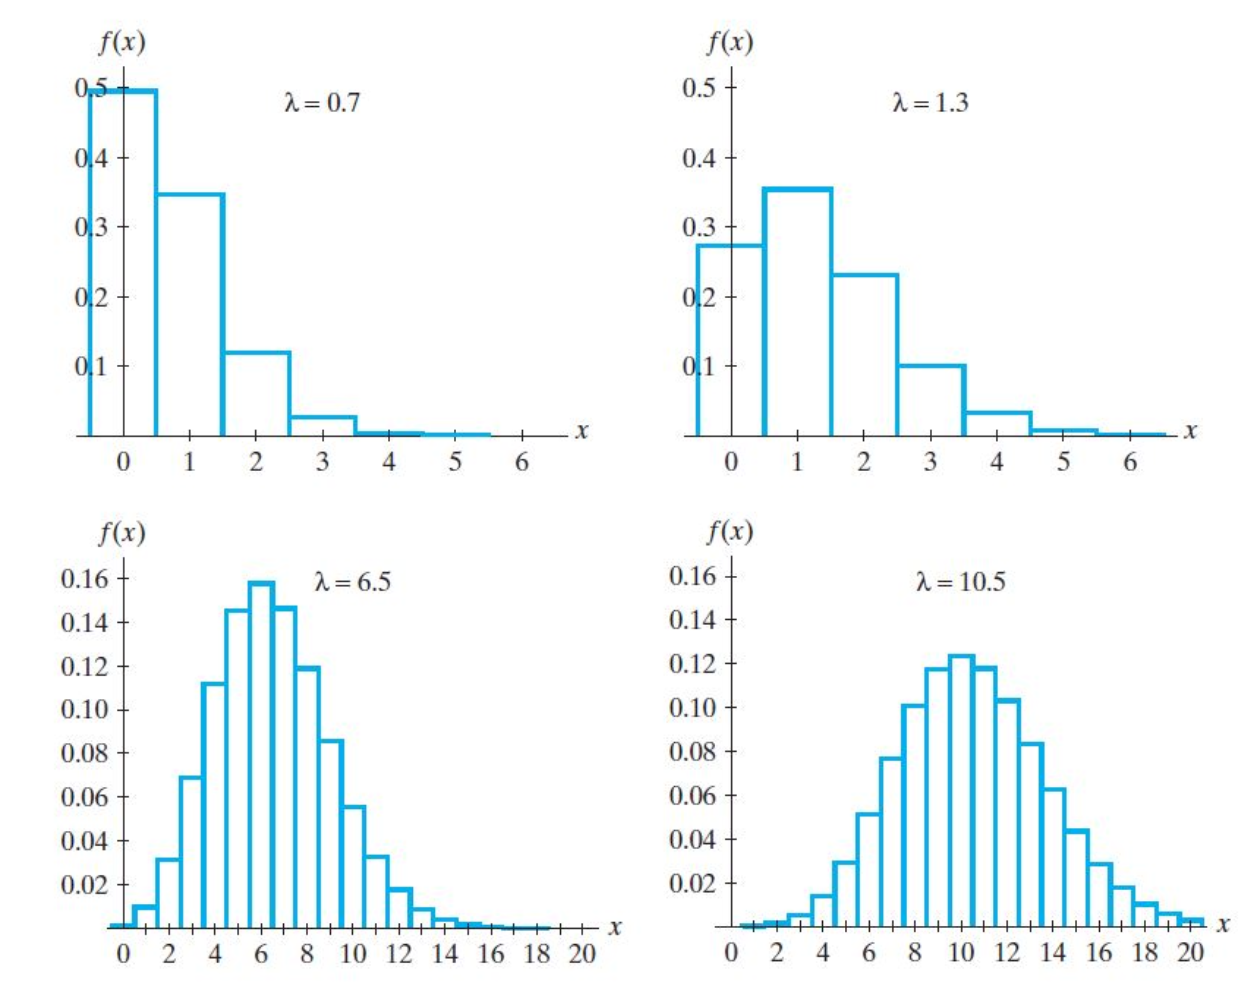
\includegraphics[scale=0.35]{test-3/poisson-pmfs}
\end{figure}

Poisson approximation to the binomial distribution\bigskip
\begin{itemize}
    \item In grad school :), you will learn that Poisson is the is the limiting distribution of binomial. Said slightly more formally:
     \[\lim_{n \to \infty} \text{Binomial}(n, p = \frac{\lambda}{n}) = \text{Poisson}(\lambda = np)\]
     \item This means that for large $n$ and small $p$, the Poisson distribution can be used to approximate the binomial distribution.
\end{itemize}\bigskip

\begin{figure}[H]
    \center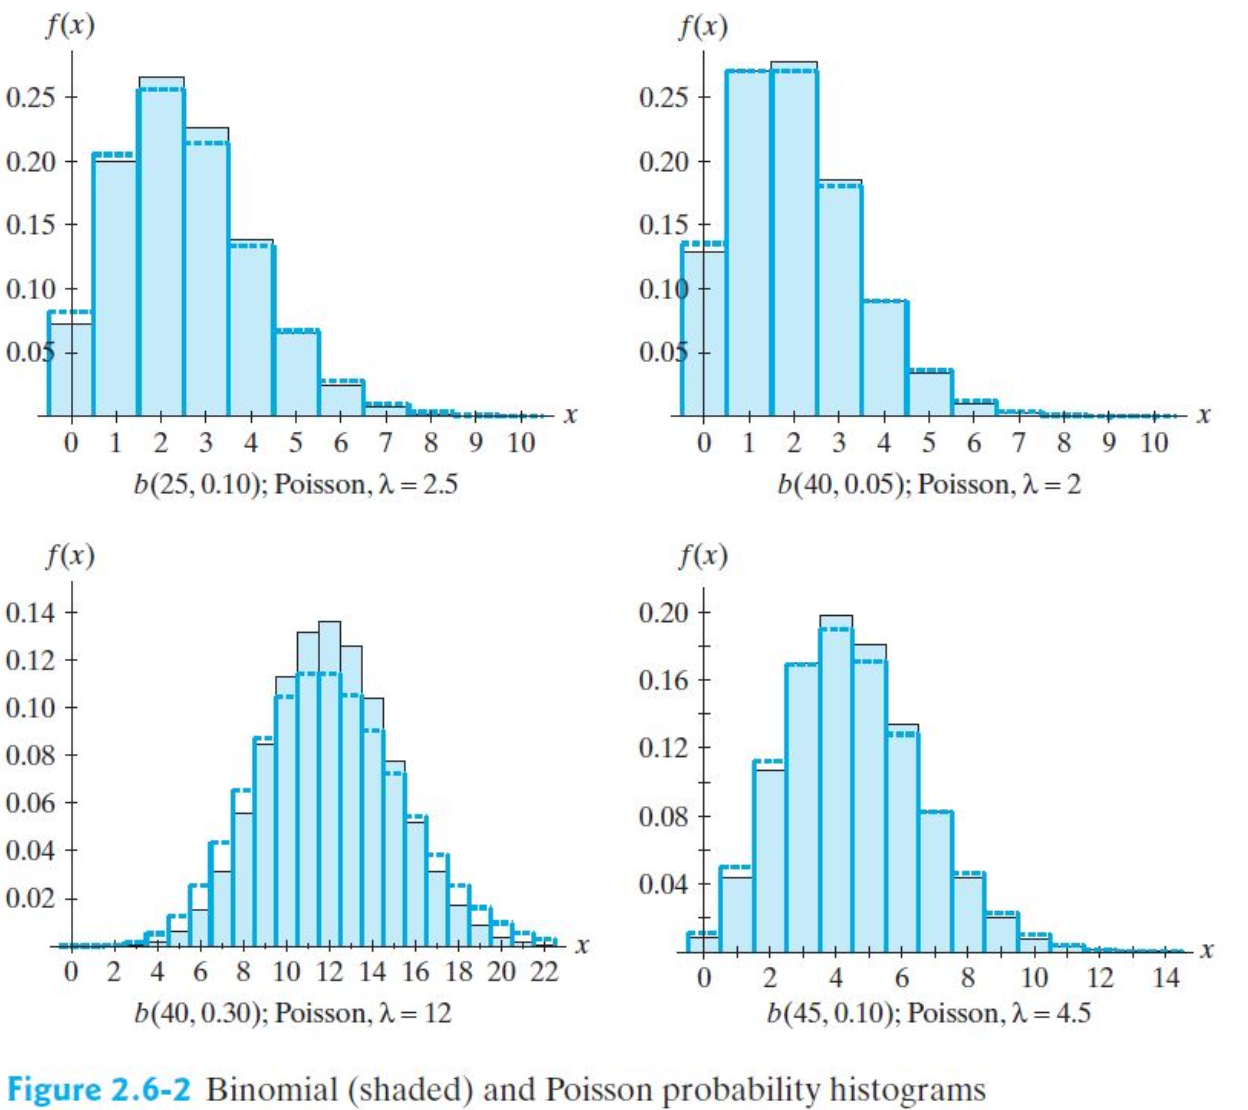
\includegraphics[scale=0.35]{test-3/poisson-approximation-to-binomial}
\end{figure}
\newpage




\end{document}